\documentclass{article}
\usepackage[utf8]{inputenc}
%%%%%%%%%%%POUR LES ALGOS %%%%%%%%%%%%%%
\usepackage [french,onelanguage,algoruled]{algorithm2e}

%%%%%%%%%%%%%%%%%%flow charts%%%%%%%%%%%%%
\usepackage{tikz}
\usetikzlibrary{shapes.geometric, arrows}
\tikzstyle{startstop} = [rectangle, rounded corners, minimum width=3cm, minimum height=1cm,text centered, draw=black, fill=red!30]
\tikzstyle{io} = [trapezium, trapezium left angle=70, trapezium right angle=110, minimum width=3cm, minimum height=1cm, text centered, draw=black, fill=blue!30]
\tikzstyle{process} = [rectangle, minimum width=3cm, minimum height=1cm, text centered, draw=black, fill=orange!30]
\tikzstyle{decision} = [diamond, minimum width=3cm, minimum height=1cm, text centered, draw=black, fill=green!30]
\tikzstyle{arrow} = [thick,->,>=stealth]
%%%%%%%%%%%%%fin%%%%%%%%%%%%%%%%%%%%%%%%%%

%%%%%%%%%%%%%%%%pour le code%%%%%%%%%%%%%%%%%
\usepackage{listings}
\usepackage{color}
%New colors defined below
\definecolor{codegreen}{rgb}{0,0.6,0}
\definecolor{codegray}{rgb}{0.5,0.5,0.5}
\definecolor{codepurple}{rgb}{0.58,0,0.82}
\definecolor{backcolour}{rgb}{0.95,0.95,0.92}

\lstdefinestyle{mystyle}{
  backgroundcolor=\color{backcolour},   commentstyle=\color{codegreen},
  keywordstyle=\color{magenta},
  numberstyle=\tiny\color{codegray},
  stringstyle=\color{codepurple},
  basicstyle=\footnotesize,
  breakatwhitespace=false,         
  breaklines=true,                 
  captionpos=b,                    
  keepspaces=true,                 
  numbers=left,                    
  numbersep=5pt,                  
  showspaces=false,                
  showstringspaces=false,
  showtabs=false,                  
  tabsize=3
}

%"mystyle" code listing set
\lstset{style=mystyle}

%%%%%%%%%%%%%%%%fin%%%%%%%%%%%%%%%%



\title{TER}
\author{jeremy.simione }
\date{April 2019}


\begin{document}

\begin{titlepage}

\begin{center}
\vspace*{-1in}
\begin{figure}[htb]
\begin{center}
%\includegraphics[width=8cm]{logo}%
\end{center}
\end{figure}

FACULTE DES SCIENCES - Année 2018-2019\\
\vspace*{0.15in}
DEPARTEMENT INFORMATIQUE \\
\vspace*{0.4in}
\begin{large}
Rapport de projet TER \\
Projet Informatique HLIN405\\
\end{large}
\vspace*{0.2in}
\begin{Large}
\textbf{Projet Sudoku en Réalité Augmentée} \\
\end{Large}
\vspace*{0.3in}
\begin{large}
Encadrant:
Boudet Vincent
 \\
\end{large}
\vspace*{0.3in}
\rule{80mm}{0.1mm}\\
\vspace*{0.1in}
\begin{large}
Etudiants: \\
Simione Jérémy, Henriksen Leif \\
 
\end{large}
\end{center}
\end{titlepage}

\newcommand{\CC}{C\nolinebreak\hspace{-.05em}\raisebox{.4ex}{\tiny\bf +}\nolinebreak\hspace{-.10em}\raisebox{.4ex}{\tiny\bf +}}
\def\CC{{C\nolinebreak[4]\hspace{-.05em}\raisebox{.4ex}{\tiny\bf ++}}}

\tableofcontents
\newpage

\section{Introduction}

\subsection{Objectifs du projet et cahier des charges}
L’objectif est de permettre à un utilisateur de prendre une photo d'une grille de Sudoku afin qu'il puisse 
obtenir la solution de la grille, le second objectif est qu'il puisse jouer sur l'application.

Il existe déjà des applications Android capables de réaliser cet objectif, mais la plupart ont du mal a obtenit un résultat correct.


Voici le cahier des charges que nous avons crée pour notre application :\\

\textbf{ Création d'un algorithme de résolution}\\
Création d'une classe Sudoku qui va représenter notre grille de sudoku mais aussi toutes les méthodes qui vont nous permettre de récuperer la grille ainsi que l'algorithme de résolution d'une grille.\\

\textbf{Création de l'interface graphique de l'application}\\
L'interface graphique nous permettra de utiliser l'application en appuyant sur des boutons.
Nous allons créer une classe Grille qui prend une grille en entrée qui vient de l'algorithme de résolution ou de l'analyse d'image et qui va l'afficher sur l'application. Cette classe Grille nous permettra d'utiliser notre grille.
\\

\textbf{Mise en place d'un accès a la caméra}\\
Création d'une classe dédiée à la caméra pour que l'utilisateur puisse prendre des photos d'une grille.
Cette partie nous servira a envoyer l'image a notre derniere partie.\\

\textbf{Mise en place d'un système d'analyse d'images}\\
Création de différentes classes qui vont nous servir à traiter l'image en utilisant la bibliothèque OpenCV
et ainsi pouvoir procéder à une reconnaissance des chiffres et l'afficher sur la grille de l'application dans le cas ou l'utilisateur voudrait résoudre une grille ou jouer.\\

\textbf{Création du jeu}\\
Création d'une partie jouable en utilisant l'interface graphique de l'application ainsi que la classe Sudoku.\\

\textbf{Rassemblement des différentes parties}\\
S'assurer de la compatiblite de tous les classes pour avoir le comportement dessire, et faire les modifications necessaires à la interface graphique pour pouvoir accerder a tous les fonctionalites de l'application.














\newpage
\section{Organisation du projet}
\subsection{Organisation du travail}
Pour le développement de notre application Sudoku , nous avons décidé de travailler chacun de notre côté et de temps en temps ensemble suivant la difficulté des choses à réaliser.Pour que le projet nous apporte a tous des connaissances dans les différents domaines auquel il touche nous avons essayé de repartir les tâches de sorte a ce que chaque membre du groupe ai vu chaque domaine (android,java,openCV).\\\\
Afin d’être les plus efficace et d’avancer le plus rapidement possible nous nous sommes réunis
quotidiennement. Durant les jours de la semaine, nous nous sommes vus souvent afin de connaître l'avancée de chacun dans le projet,faire le point sur l’avancement du projet, définir de nouveaux objectifs et de les réaliser.\\\\
A chaque étape réalisée nous avons postés sur un depot Github créé pour le projet chaque nouvelle partie afin que tout chaque memebre puisse s'informer et voir.
A chaque étape importante nous nous sommes réunis avec notre encadrant M. Boudet afin de faire le point sur l’état d’avancement de l’application.\\\\

\subsection{Répartition du travail dans le temps}

Nous avons découpé cette période de travail en plusieurs phases.
\begin{enumerate}
    \item Préparation du projet. Nous avons réalisé le cahier des charges de l’application, choisi les
          outils de travail et les principales technologies utilisées. Nous avons fait une première version
          du diagramme de répartition des tâches dans le temps, et une première modélisation de
          l’architecture de l’application.
\item Développement du projet. Nous avons implanté les fonctionnalités de l’application en
raffinant la modélisation au fur et à mesure. Pour chaque module implanté, nous nous sommes
efforcés d’écrire des tests afin de s’assurer de leur bon fonctionnement.
\item Finalisation du projet. Cette phase a consisté en la correction de bogues afin d’obtenir une
version suffisamment stable pour pouvoir être présentée en vue de la soutenance et du rendu
du projet T.E.R.
\end{enumerate}
\newpage

\subsection{Outils de travail collaboratif }
Nous avons choisi d’utiliser Github qui  permet la gestion des versions du projet et facilite la collaboration a distance.\\\\
Enfin, pour éditer le code du projet , nous nous sommes servis d'Android Studio.\\\\
Il etait en effet plus facile de commencer sur cet éditeur car il ne fonctionne pas de la meme facon que les autres éditeurs et notre code source final passe obligatoirement par cet IDE.
Nous avons aussi créer un diagramme de gantt afin de planifier les tâches pour avoir des dates limites pour chaque partie ce qui nous a permis de réaliser le projet dans son ensemble et dans les temps.\\
\newline Pour rédiger les différents documents, y compris ce rapport, nous
avons utilisé \LaTeX  pour sa capacité à produire des documents de bonne qualité.


\section{Conception}

Nous avons décidé de faire la conception de ce projet en 5 parties, analyse d'image, interface graphique et interaction, le jeu, algorithme de résolution, et rassemblement des parties. Nous avons essayé d'avoir une intersection vide entre les 5 parties, avec le but de pouvoir travailler parallèlement, donc à part la partie rassemblement et interface graphique avec jeu, les différents parties sont indépendants. 
\\
\\
Tout d'abord nous allons vous expliquer l'idée générale de notre application, comment elle fonctionne et ses objectifs, puis nous allons décrire avec plus de détails les 5 parties mentionnées précédemment dans l'ordre suivant, premièrement l'analyse d'image, deuxièmement l'interface graphique et l'interaction, troisièmement l'algorithme de résolution, quatrièmement le jeu, et cinquièmement le rassemblement des parties.




\subsection{General}

Notre application à pour but de prendre en photo une grille de sudoku, analyser cette image, extraire les valeurs des cases et les affiches dans une grille, une fois les valeurs sont dans l’application, on peut choisir de jouer ou de résoudre la grille en utilisant l’algorithme de résolution. 



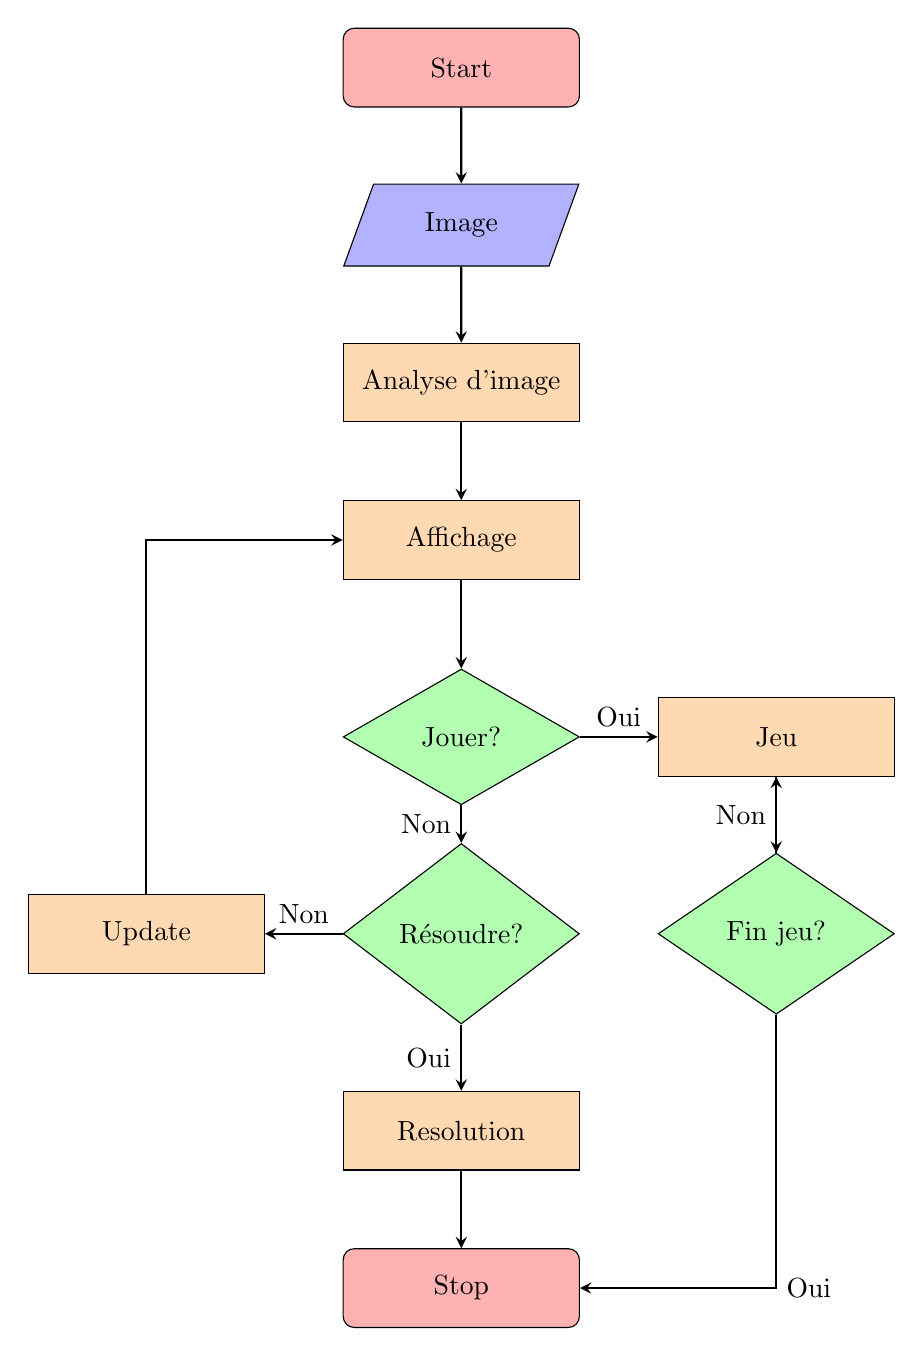
\begin{tikzpicture}[node distance=2cm]
\node (start) [startstop] {Start};
\node (in1) [io, below of=start] {Image};
\node (pro1) [process, below of=in1] {Analyse d'image};
\node (pro2) [process, below of=pro1] {Affichage};
\node (dec1) [decision, below of=pro2, yshift=-0.5cm] {Jouer?};
\node (pro2a) [process, right of=dec1, xshift=2cm] {Jeu};
\node (dec1a) [decision, below of=pro2a, yshift=-0.5cm] {Fin jeu?};
\node (dec2) [decision, below of=dec1, yshift=-0.5cm] {Résoudre?};

\node (pro3) [process, below of=dec2
, yshift=-0.5cm] {Resolution};

\node (pro4) [process, left of=dec2, xshift=-2cm] {Update};

\node (stop) [startstop, below of=pro3] {Stop};

\draw [arrow] (start) -- (in1);
\draw [arrow] (in1) -- (pro1);
\draw [arrow] (pro1) -- (pro2);
\draw [arrow] (pro2) -- (dec1);
\draw [arrow] (pro2a) -- (dec1a);
\draw [arrow] (dec1) -- node[anchor=south] {Oui}(pro2a);
\draw [arrow] (dec1a) -- node[anchor=east] {Non}(pro2a);
\draw [arrow] (dec1a) |- node[anchor=west] {Oui}(stop);
\draw [arrow] (dec1) -- node[anchor=east] {Non}(dec2);
\draw [arrow] (dec2) -- node[anchor=east] {Oui}(pro3);
\draw [arrow] (dec2) -- node[anchor=south] {Non}(pro4);

\draw [arrow] (pro4) |- (pro2);
\draw [arrow] (pro3) -- (stop);
\end{tikzpicture}
\\
\subsection{Analyse d'image}
\subsection{Interface graphique et interaction}
L’interface graphique est divisé en deux components principales, d’abord la grille de 81 cases, et après, les boutons nécessaires à l'utilisation de l’application. La deuxième partie est simplement une interface de menu classique, différentes boutons qui donneront accès aux autres parties de l’application. La première partie est chargée de l’affichage des données qui vient de l’analyse d’image ou de l'algorithme de résolution, et aussi est charge de permettre à l'utilisateur de modifier les valeurs des casses, pour qu'il puisse modifier la grille s’il y a eu un erreur avec l’analyse d’image ou s’il a choisi de jouer. Donc elle est beaucoup plus compliqué et nous allons l’expliquer plus en détaille.
\\
\\
Nous avons créé 4 classes pour  mettre en place la grille, 

\begin{itemize}
    \item EditeurGrille \\
La classe EditeurGrille est chargée de gérer les valeurs qui viennent de l’analyse d’image et l’algorithme de résolution, aussi du control des boutons pour la modification des valeurs. 

    \item Grille \\
La classe Grille contient tout les méthodes nécessaires pour faire la mise à jour de la grille, Grille lit les couleurs des casses, le nombre de chaque casse, et les affiche correctement.
    
    \item Cases \\
La classe Cases contient 81 objets Case, et elle est chargée de les modifier tous ensemble et les gérer. 
    
    \item Case \\
La classe Case représente une casse dans la grille, elle contient plusieurs attributs utiles pour l'éditeur et pour le jeu, principalement une Case contient une valeur et une couleur(blanc, bleu ou rouge), le couleur blanc représente une casse modifiable, bleu une casse non modifiable (si on n’est pas en mode jeu on peut toujour modifier une casse bleu), et rouge une casse avec une mauvaise valeur (utilisée seulement dans le jeu) . Case contient aussi autres attributs et méthodes mais ils seront expliqué avec plus de détaille dans la partie Jeu.


\end{itemize}\\


\subsection{Algorithme de resolution}
\subsection{Jeu}
Pour le jeu nous avons créé la classe Jouer qui hérite de la classe EditeurGrille, le jeu fait la même chose que EditeurGrille, mais utilise des attributs dans la classe Case pour la logique de jeu. La classe Case contient deux attributs importants pour le jeu, estModifiable et valeurReponse,  quand nous essayons de changer la valeur d’une casse d’abord nous vérifions si elle est modifiable, après nous confirmons si nous avons mis la bonne valeur, si c'était le cas nous la transformons en non modifiable, nous changeons la valeur et la couleur en bleu et nous enlevons 1 au compteur de casses vides, sinon nous changeons la couleur en rouge et ajoutons 1 au compteur d’erreurs. Le jeu finit quand le nombre de cases vides est equal a 0.

\subsection{Rassemblement}
Pour le rassemblement nous nous avons assurer que les autres parties étaient le plus indépendantes possibles, donc pour les rassembler nous avons utilisé les outils de notre système d'exploitation, Android, pour qu’elles puissent communiquer entre elles, et grâce à leur indépendance nous avons évité centaines de bugs. L’analyse d’image envoi de l’information à l'éditeur de grille, puis si le joueur souhaite la résolution, l’algorithme de résolution lui donne la réponse, sinon l'éditeur de grille envoi l’information de la grille à la classe Jouer, et le joueur peut jouer.



\section{Implémentation du Sudoku}

\subsection{Création de l'algorithme de résolution}

La première partie consistait a créer une classe java de sudoku pour pouvoir implémenter la résolution; la solution la plus simple était de choisr une structure de données de type tableau.
\newline
\newline La deuxième étape consitait a créer des fonctions secondaires qui nous servirait pour la résolution de la grille entière; nous avons donc créer des fonctions qui testent si une valeur est absente d'un bloc, d'une colonne ou d'une ligne de la grille ; voici un exemple de l'une de ces fonctions:\\


\begin{algorithm}[H]
\SetAlgoLined
\KwData{Entier valeur,Grille grille,Entier j}
\KwResult{Renvoi vrai si la valeur n'est pas dans la colonne, faux sinon }
\For{i allant de 0 à 9}{
        \If{grille[i][j]=k}{
        \Return{Faux}
        }
        \Elf{
        \Return{Vrai}
    }
}
\caption{absentSurColonne(Entier valeur,Grille g,Entier j)}
\end{algorithm}\\\\


La troisième étape consistait à implémenter le backtrack\footnote{Aussi nommé le retour sur trace en français}.Cette fonction doit prendre une grille en entrée la résoudre et nous informer de l'état du réultat en nous renvoyant un booléen.
Il fallait donc vérifier dans la descente récursive en énumérerant tous les chiffres possibles pour observer si nous arrivions à un résultat correct ou un blocage tout cela en remplissant la grille dans la descente et si nous arrivions à un blocage nous reinitialisions la case correspondante à zéro.\\
Voici l'algorithme en question :


\begin{algorithm}[H]
\SetAlgoLined
\KwData{Grille grille,Entier position}
\KwResult{Renvoi vrai si la grille a été résolue, renvoi faux sinon}
\If{position=9*9}{\Return{Vrai} }
$i \longleftarrow position \div 9  $
$j \longleftarrow position \% 9$\\
\If{grille[i][j]!=0}{\Return{estValide(grille,postion+1);\\
\For{k allant de 1 à 9}{
\If{absentSurLigne(k,grille,i) et absentSurColonne(k,grille,j) et absentSurBloc(k,grille,i,j)}{grille[i][j] \longleftarrow k;\\
\If{estValide(grille,position+1)}{\Return{Vrai}}}
$grille[i][j] \longleftarrow 0$\\
\caption{estValide(Grille grille,Entier position)}
\Return{Faux}
}
}
}
\end{algorithm}\\

\subsection{Mise en place d'un système de reconnaissance des chiffres}
Pour réaliser le système de reconnaisance des chiffres, nous avons du utiliser la bibliothèque graphique OpenCV.
La plupart des problèmes que nous pouvons rencontrer avec cette bibliothèque ne sont très bien documentés car c'est une bibliothèque technique et utilisé surtout par des gens qualifiés.\\\\
Nous avons opté pour une implémentation permettant d'afficher sur une grille la reconnaissance d'une image provenant d'un traitement.Le but est que du moment ou l'image a été traitée elle est directement envoyé a l'IA pour qu'elle soit ensuite directement affichée sur l'application.\\

Lorsque l'utilisateur va sélectionner l'image elle sera directement envoyé au programme de traitement de l'image qui lui-même envera le résultat a l'IA qui essaiera de reconnaitre les chiffres puis d'envoyer un résultat a la classe Sudoku qui l'affichera par la suite.\\

Pour cette partie nous avons décider de nous faciliter la tâche en utilisant l'IDE eclipse car la gestion des chemins d'accès des images\footnote{En effet lors de la création d'une application Android les chemin d'accès aux images doivent provenir exclusivement du téléphone.} était plus aiséé et ainsi pouvoir observer les traitements résultants afin d'obtenir une image lisible par l'ordinateur.\\
\\

Pour implémenter ce traitement il y avait un cahier des charges à suivre :

Premièrement il fallait détecter la grille en appliquant une série de traitements à l'image a savoir:
\begin{itemize}
    \item Convertir notre image de base avec des teintes grises
    \item Appliquer un flou gaussien afin de réduire le bruit et les détails de l'image
    \item Appliquer un seuillage d'image c'est a dire convertir notre résultat précedant en noir et blanc
    \item Trouver les bordures de la grille
    \item Détecter les lignes de la grille
\end{itemize}\\

Voici ci-dessous des algorithmes de traitement de l'image utilisés par OpenCV:

Il fallait créer ensuite un système d'intelligence artificielle qui  allait essayer de comparer chaque chiffre de la grille avec des ressources et renvoyer une grille en résultat.

La derniere partie consistait a lier les trois classes c'est a dire notre classe Sudoku, celle qui manipulait l'image et l'intelligence artificielle et adapter notre code afin qu'il soit effectif sur un terminal android.

Voici ci-dessous des algorithmes de traitement de l'image utilisés par OpenCV:

\newpage
%%%%%%%%%%%%%%%partie leif%%%%%%%%%%%%%%%%%%%%%%%%%%%%%
\subsection{Interface graphique}
\subsubsection{XML et boutons}
Tous les Activitys de Android ont un fichier XML ou est décrit leur apparence, dans le XML est décrit la position, taille, couleur, et autres caractéristiques des boutons, balises de texte etc.
\begin{lstlisting}[language=Java, caption = Exemple balise XML] 

        <Button
            android:id="@+id/button5"
            android:layout_width="50dp"
            android:layout_height="wrap_content"
            android:text="5"/>


\end{lstlisting}
Pour la grille nous avons utilisé la balise GridView, nous allons expliquer plus en dettaille cette balise dans la partie EditeurGrille, pour les boutons nous avons utilise la balise button, chaque button dans le XML contient different attributs pour modifier leur position et apparence, mais l’attribut le plus importante c’est le “id”, l’id nous permettra de utiliser le bouton application. Pour utiliser le nous modifions le fichier Java de notre activité et créons un méthode a exécuter quand nous touchons le bouton, 

\begin{lstlisting}[language=Java, caption = Méthode du bouton] 

void click(){
//code
}

\end{lstlisting}

et dans le XML, dans la balise bouton nous ajoutons 

\begin{lstlisting}[language=Java] 
android:onClick="click"

\end{lstlisting}

alors a chaque fois que on touche le bouton nous allons exécuter le code qui est dans click.
Il y a une autre façon de faire aussi, dans le fichier Java nous créons une instance Button, 
pour activer le bouton et décrire son comportement après de l’avoir touché, avec cette méthode nous utilisons l'id pour différencier les boutons.
\begin{lstlisting}[language=Java, caption=Initialisation d'un bouton] 

Button notreBouton= findViewById(R.id.notreBouton);  
notreBouton.setOnClickListener(new View.OnClickListener() {
    public void onClick(View v) {
        // Code a executer
    } 
});

\end{lstlisting}
Les deux méthodes marchent mais la deuxième devient très verbeux si nous avons trop de boutons.
\subsection{La grille}
\subsubsection{Classe Case}
Chaque instance de une Case represente une casse dans la grille, chaque Case contient quatre attributs, estModifiable, couleur, valeur, et valeurReponse.
\\
\\
estModifiable est un boolean, si il est vrai la casse est modifible sinon elle ne l’est pas.
\\
\\
couleur est un entier entre 0 et 2, 0 est le blanc et represent que une case est vide et modifiable, 1 est le bleu et represente que une casse est non modifiable et elle contient la valeur de la réponse, 2 est le rouge et 
représente qu'une casse a une valeur différente à la valeurReponse.
\\
\\
valeur est la valeur courante de la casse, et elle est la valeur que  nous affichons.
\\
\\
valeurReponse est un attribut caché, il contient la valeur de la réponse de une case, il est utilisé pour le jeu, pour savoir si le jouer c’est trompe.

\subsubsection{Classe Cases}
La classe Cases est utilise pour stocker les 81 cases de la grille, accéder aux casses en utilisant la méthode getCaseAt(), et montrer la réponse de la grille en utilisant montrerReponse() qui change la valeur des cases pour la valeur de leur réponse. 
\\
\\
\begin{lstlisting}[language=Java, caption = Méthode pour le remplissage de cases] 

public void initJeu(List<String> vals, List<String> valsResolution) {
 int x = 0;
       
 //9 lignes
 for (int i = 0; i < 9; i += 3) {
    //3 lignes
    for (int e = 0; e < 3; e++){
    //une lignes
        for (int k = i; k < (i + 3); k++) {
            for (int j = x; j < (x + 3); j++) {
                if(vals.get(j).equals(""))
                    cases.get(k).add(new Case(true, vals.get(j), valsResolution.get(j)));
                        else
                    cases.get(k).add(new Case(false, vals.get(j), valsResolution.get(j)));
                }
                    x = x + 3;
            }
        }
    }
}
\end{lstlisting}
\\
Dans le listing 4, nous pouvons voir l'algorithme de remplissage, il prend comme entre les valeurs de la grille et les valeurs de résolution, notre grille ressemble une tableau de deux dimensions mais elle est une liste de liste, ou chaque liste représente une grille 9x9, pour bien remplir la liste cases nous allons changer de grille 9x9 tous les trois éléments.
\\
\\
Par exemple si nous utilisons boucle normal le résultat c'est celui la,
\begin{center}
\begin{tabular}{ c c c c c c}
 0 & 1 & 2 & 9 & 10 & 11\\ 
 3 & 4 & 5 & 12 & 13 & 14\\  
 6 & 7 & 8 & 15 & 16 & 17  
\end{tabular}
\end{center}
\\
notre grille est représente par une liste de Strings donc si on veut la valeur de la position 6 on reçoit la valeur 3 au lieu de 6.
\\
\\
Avec notre algorithme résultat c'est celui la,
\begin{center}
\begin{tabular}{ c c c c c c}
 0 & 1 & 2 & 3 & 4 & 5\\ 
 6 & 7 & 8 & 9 & 10 & 11 \\  
 12 & 13 & 14 & 15 & 16 & 17  
\end{tabular}
\end{center}
\\
ce méthode, évidement difficile a comprendre, nous permettra de utiliser la grille avec le numéro de la dernier GridView touche, et la position touche dans celui la pour accéder et modifier la bonne casse, .

\subsubsection{Classe Grille}
La classe Grille est charge de la manipulation des GridViews. Elle contient une instance de Cases pour stocker l'information des casses.

\begin{itemize}

\item{GridView}
\\
\\
Une GridView prend une liste, dans notre cas un Array liste, après la GridView utilise les informations de la liste et les affiche en deux dimension, avec le nombre de colonnes donnés dans le XML. La liste peut avoir images, texte, ou autres, dans notre cas nous avons utilisé texte donc nous créons des TextViews dans setAdapter, et la GridView affichera les TextViews en forme de Grille.

\begin{lstlisting}[language=Java, caption = Exemple setAdapter] 
gv.setAdapter
(new ArrayAdapter<String>(activity, android.R.layout.simple_list_item_1, numbers.get(0))
{
public View getView(int position, View convertView, ViewGroup parent) {

// Return the GridView current item as a View
View view = super.getView(position,convertView,parent);

// Convert the view as a TextView widget
TextView tv = (TextView) view;

//tv.setTextColor(Color.DKGRAY);

                
RelativeLayout.LayoutParams lp =  new RelativeLayout.LayoutParams(
LinearLayout.LayoutParams.MATCH_PARENT, LinearLayout.LayoutParams.MATCH_PARENT
);
    
tv.setLayoutParams(lp);

// Get the TextView LayoutParams
RelativeLayout.LayoutParams params = (RelativeLayout.LayoutParams)tv.getLayoutParams();

tv.setLayoutParams(params);

// Display TextView text in center position
tv.setGravity(Gravity.CENTER);

tv.setPadding(0,0,0,0);

//set valeur
tv.setText(cases.getCaseAt(0,position).getValeur());
                
// Set the TextView background color
if(cases.getCaseAt(0,position).getCouleur() == 0) {
    tv.setTextColor(Color.parseColor("black"));
    tv.setBackgroundColor(Color.parseColor("white"));
}
else if(cases.getCaseAt(0,position).getCouleur() == 1) {
    tv.setBackgroundColor(Color.parseColor("grey"));
    tv.setTextColor(Color.parseColor("white"));
}
else
    tv.setBackgroundColor(Color.parseColor("red"));
               
return tv;
}
});
\end{lstlisting}
\item{Liste vers liste de listes}
\\
\\
La grille ressemble une mais en vrai c’est une liste de liste, donc pour accéder à une casse nous avons besoin du nombre de la Gridview et de la position dans la GridView.  Grâce au constructeur de Cases, le  listes ont la bonne valeur par exemple la casse 3 de la grille 1 représente la casse 9 de la liste et non pas la casse 3. Dans la partie difficultés nous allons expliquer pourquoi nous l'avons fait de ce manière la.

\item{onClick}
\\
\\
L'onClick de la classe Grille change la valeur de la dernier grille sélectionnée, la dernière position, la couleur de la casse en vert, et remet l'ancien casse touche à son couleur de base. 



\begin{lstlisting}[language=Java, caption = Exemple d'une methode dans onclick] 
case R.id.gv9: {
if(activity.getPreviousSelectedGridView() == -1)                    
    activity.setPreviousSelectedGridView(9);
else if(activity.getPreviousSelectedGridView() != 9)
    getGv(activity.getPreviousSelectedGridView()).invalidateViews();

activity.setPreviousSelectedGridView(9);

// Get the GridView selected/clicked item text
String selectedItem = parent.getItemAtPosition(position).toString();

//prendre la cellule actuelle
TextView tv2 = (TextView) view;

tv2.setBackgroundColor(Color.parseColor("#FF9AD082"));

// Display the selected/clicked item text and position on TextView
//tv.setText("GridView item clicked : " +selectedItem + "\nAt index position : " + position);

TextView previousSelectedView = (TextView) gv9.getChildAt(activity.getPreviousSelectedPosition());

// If there is a previous selected view exists
if (position != activity.getPreviousSelectedPosition()) {
    if (activity.getPreviousSelectedPosition() != -1) {
        // Set the last selected View to deselect
        previousSelectedView.setSelected(false);
        switch (cases.getCaseAt(8,activity.getPreviousSelectedPosition()).getCouleur())
            {
                case 0:
                 previousSelectedView.setBackgroundColor(Color.parseColor("white"));
                break;
                case 1:
                 previousSelectedView.setBackgroundColor(Color.parseColor("grey"));
                break;
                case 2:
                 previousSelectedView.setBackgroundColor(Color.parseColor("red"));
                break;
            }
        // Set the last selected View text color as deselected item
        //previousSelectedView.setTextColor(Color.DKGRAY);
        }

        // Set the current selected view position as previousSelectedPosition
        activity.setPreviousSelectedPosition(position);
    }
}
\end{lstlisting}






\item{invalidateViews}
\\
\\
On utilisé la méthode invalidateViews pour mettre à jour tous les grilles à jour. 
\end{itemize}

\subsubsection{Classe EditeurGrille}
L’EditeurGrille est une activity, elle est charge d'initialiser la classe Grille et la classe Cases, puis les rassembler, elle est aussi chargée de gérer les boutons et leurs actions. EditeurGrille étant une activity possède un fichier XML, le fichier XML est composé de 3 LinearLayouts horizontales avec 3 GridView de dans, chaque GridView représente un carré 3x3 dans la grille, nous avons fait 9 GridView séparés pour pouvoir avoir de colonnes et lignes gras séparant les sections.  Après a la fin de le XML on trouve les boutons de 1 à 9, un bouton pour effacer, jouer et résoudre la grille.

\begin{itemize}
    \item{onCreate}
    \\
    \\
    La méthode onCreate c'est la premier méthode qui s'exécute dans l'Activity, donc EditeurGrille fait les étapes suivantes:
    
    \begin{itemize}
        \item Récupérer le String donne par l'analyse d'image, nous allons détailler cette partie dans la partie rassemblement.
        \item Initialiser les listes grilleAsList et grilleResolu.
        \begin{lstlisting}[language=Java, caption = Initialisation listes] 
grilleAsList = new ArrayList<String>(Arrays.asList(str));
grilleResolu = new ArrayList<String>(Arrays.asList(str));
        \end{lstlisting}
        \item Utiliser la méthode setAdapters avec grilleAsList.
        \item Résoudre grilleResolu que avant avait les mêmes valeurs que grilleAslist.
        \item Initialiser une instance de Cases pour l'attribut grilles qui est une instance de Grille.
        \item Initialiser le itemClickListener pour grilles.
        \begin{lstlisting}[language=Java, caption = Initialisation itemClickListener] 
itemClickListener = new AdapterView.OnItemClickListener() {
    @Override
    public void onItemClick(AdapterView<?> parent, View view, int position, long id) {
      grilles.click(parent, view, position, id, activity);
    }
};
        
grilles.setClickListeners(itemClickListener);
\end{lstlisting}
    
    \end{itemize}
    \item{onClick}
    \\
    \\
    La methode onCLick d'EditeurGrille est charge de modifier les valeurs de la grille dans le cas ou l'analyse d'image se soit trompe, ou de montrer la résolution en utilisant la méthode motrerReponse de Cases.
   \begin{lstlisting}[language=Java, caption = Exemple onClick EditeurGrille] 
case R.id.button4:
if(previousSelectedPosition != -1 && Sudoku.positionValide(Sudoku.listToArr(grilleAsList), 4, grilles.getPoints(posGrille).x, grilles.getPoints(posGrille).y))
{
  grilleAsList.set(grilles.getPositionGrille(previousSelectedGridView - 1, previousSelectedPosition), "4");
  cases.getCaseAt(previousSelectedGridView-1,previousSelectedPosition).setValeur("4");
}
else
{
  Toast toast = Toast.makeText(getApplicationContext(),"Numero NON valide", Toast.LENGTH_LONG);
  toast.setGravity(Gravity.CENTER, 0, 0);
  toast.show();
  }
grilles.refreshNumbers(grilleAsList);
grilles.invalidateViews();
break;
    \end{lstlisting}

\end{itemize}

\subsection{Jeu}
Pour le jeu nous avons fait une classe qui herite de EditeurGrille, nous avons ajoute deux attributs casesVides et nbErreurs, si casesVides est egal à 0, alors le jeu c'est fini et nous changeons d'Activity, aussi si nbErreurs est superior à 10, le jeu fini.
\\
\\
Nous avons modifie aussi l'onClick, nous révisons si le nombre choisi c'est le bon, si la réponse est oui, nous  soustrayons 1 à casesVides, changeons la case à non modifiable et changeons la couleur, sinon nous ajoutons 1 à nbErreurs et changeons de couleur.

\subsection{Rassemblement}
Pour le rassemblement nous avons mélange tout les Activitys, le menu principal, l'analyse d'image, l'éditeur de grille et le jeu. Pour cela nous avons d'abord ajouter tous les Activitys au manifeste, apres pour creer une autre Activity dans une Activity, nous creons un Intent de la manier suivante,
\begin{lstlisting}[language=Java, caption = Creation Intent] 
Intent intent = new Intent(this, NouvelleActivity.class);
\end{lstlisting}
\\
apres pour passer de l'information à l'autre Activity nous écrivons le code suivante,
\begin{lstlisting}[language=Java, caption = Envoyer un String[]] 
intent.putExtra("EXTRA_MESSAGE", str);
\end{lstlisting}
\\
dans notre cas nous envoyons un String[] appelé str, avec l'identifiant "EXTRA\_MESSAGE", pour commencer l'Activity nous faisons le suivant.
\begin{lstlisting}[language=Java, caption = Commencer une Activity] 
 startActivity(intent);
\end{lstlisting}
\\
Apres dans la nouvelle Activity, pour recouper str nous faisons une instance de Bundle et on cherche dans cette instance str, utilisant son identifiant.
\begin{lstlisting}[language=Java, caption = Récupérer une valeur] 
 Bundle extras = getIntent().getExtras();
 str2 = extras.getStringArray("EXTRA_MESSAGE");
\end{lstlisting}
\\


%%%%%%%%%%%%%%%%%%%%fin%%%%%%%%%%%%%%%%%%%%%%%%%%%%%%%%%%%%%

\section{Bilan et difficultés rencontrées}

\subsection{Avancement du projet}





\subsection{Difficultés rencontrées}

\subsubsection{Analyse d'image}
Pour la partie "Mise en place d'un systeme de reconnaissance de chiffres" nous avons été confrontés pour l la première fois a une bibliotheques de traitement d'image et la gestion d'une intelligence artificielle.\\\\
Nous avons donc du nous former a cette bibliothèque et après de nombreux essais nous nous ne savions pas si notre système d'IA allait réussir à détecter notre image traitée c'est pourquoi après concertation avec notre encadrant nous avons décidé d'utiliser une classe déja existante nommée ImageManipulator qui traitait l'image comme nous avions besoin afin d'être sûr que le résultat serait correct et que l'image sera ainsi facilement lisible par l'IA.Nous sommes donc parvenus a surmonter cette difficulté en utilisant des classes deja existantes a savoir une classe qui nous a permis de manipuler l'image et une classe qui nous a servi d'intelligence artificielle.\\

Ensuite malgré la grande aide que nous ont apportés ces deux classes l'adaptation du code d'eclipse à Android Studio a été très difficile car il fallait déjà réussir a installer une version d'openCV sur l'IDE Android ce qui n'a pas été chose aisée, mais aussi une fois ceci fait, trouver une version qui compilait à l'appel de la bibliothèque et vérifier qu'openCV était bien fonctionnel.\\
Ensuite plus rien ne fonctionnait de la même façon il a donc fallu créer des classes qui nous ont permis de passer outre cette difficulté et pouvoir faire l'adaptation à Android Studio.\\

Cette partie a été de loin la plus longue et la plus dure.

\subsubsection{Grille avec liste de liste}
Au début la Grille était représenté uniquement par une liste et un seul GridView non pas neuf, donc trouver une case spécifique était facile, mais le problème était que la grille n'avait pas de lignes et colonnes gras, donc l'expérience de l'utilisateur n'était pas très agréable car trouver les chiffres était difficile. Pour résoudre cette problème nous avons pense à utiliser des images, mais le problème était que pour neuf chiffres il nous aurait fallu 81 images, neuf images pour le milieu, neuf images pour le coin gauche en haut, etc. Alors nous avons décidé de faire les neuf GridViews, cela a marche mais nous avons pris un temps considérable pour créer l'algorithme de remplissage avec décalage et mettre tout en ordre, car le système avec la liste de listes n'est pas très intuitive.

\subsubsection{equals}
Etant habitues à coder en C++ et ayant peu d'experience avec Java, nous avons utilise == pour comparer des Strings dans plusieurs parties de notre code, donc nous avons eu beaucoup de bugs, et le problème était que n'étant pas conscients de que == ne fonctionné pas pour les String en java, nous avons dépensé un temps importante à cherche des bugs dans des autres parties du code avant de trouver que c'était le == qui ne fonctionné pas. Aujourd'hui nous avons bien compris de ne pas utiliser == pour les Strings. 

\subsubsection{Débogage avec Android}
Le débugage avec n'est pas le même que dans un terminal, dans Android Studio nous avons un log qui marche plus ou moins comme un terminal et affiche des informations soit de l'application ou d'Android. Les deux problèmes que nous avons rencontré c'est que System.out.println() ne marchait pas tout le temps, donc au début nous avons dépensé du temps a résoudre cette problème, finalement nous avons trouve la classe Log d'Android qui est faite seulement pour afficher de l'information dans le log. Après nous nous avons rendu compte que parfois l'application donne trop d'information et elle disparaissait, nous n'avons pas résolu cette problème, la seule solution que nous avons trouve c'était de débrancher le téléphone.













\end{document}